\begin{frame}{Algorithm - Alternance maillage et simulation}
    \small
    \begin{algorithm}[H]
        \SetAlgoLined
        \label{algo:iterative_meshing_quadcover}
        \KwIn{Maillage de l'état initial de l'objet $Q_0$}
        \KwOut{Un maillage par pas de temps de la simulation $(Q_n)_{n \leq N}$}
        \SetKwProg{Fn}{Function}{:}{}
        \Fn{QuadcoverIteratif($Q_0$)}{
        $n_f \gets 0$\\
        \While{$n_f < N$}{
            Lancement de la simulation de déformation sur le maillage $Q_0$.\\
            $(Q_n)_{n \leq n_f} \gets$ un maillage quadrilatère par pas de temps réussi de la simulation\\
            \ForAll{$n \leq n_f$}{
                $T_n \gets Q_n$ divisé en un maillage triangulaire\\
            }
            $Q_0 \gets$ calcul d'un maillage initial adapté aux déformations $(T_n)_{n \leq N}$\\
        }
        \Return{$(Q_n)_{n \leq N}$}
        }
    \end{algorithm}
\end{frame}
\begin{frame}{Déterminer des valences de bord adaptés à la déformation}
    \small
    \begin{figure}
        \centering
        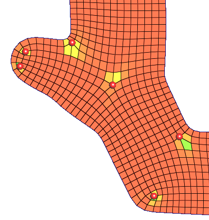
\includegraphics[width=0.46\linewidth]{img/quadsimu/coin_pb_0.PNG}
        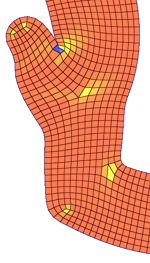
\includegraphics[width=0.27\linewidth]{img/quadsimu/coin_pb_1.PNG}
        \caption{Les positions de singularités optimales pour une géométrie initiale peuvent conduire à des quadrilatères de qualité médiocre après une déformation.}
        \label{fig:asp_ratio_pb}
    \end{figure}
\end{frame}
\begin{frame}{Déterminer des valences de bord adaptés à la déformation}
    \small
    \begin{figure}
        \centering
        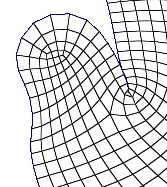
\includegraphics[width=0.39\linewidth]{img/quadsimu/coin_rs_0.PNG}
        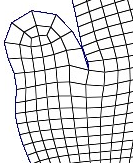
\includegraphics[width=0.35\linewidth]{img/quadsimu/coin_rs_1.PNG}
        \caption{En utilisant toutes les géométries de l'itération précédente de la simulation échouée, 4 quadrilatères adjacents sont automatiquement placés au 
        point de bord où la déformation est la plus prononcée.}
        \label{fig:asp_ratio_sol}
    \end{figure}
\end{frame}

\begin{frame}{Carte sans couture adapté à la déformation}
    On fait la moyenne des $N$ champ de repère: 
    $$ \mu_i = \frac{1}{N} \sum_{n \leq N} \mu_{i, n} $$
    \pause
    On calcule une carte sans couture $u$ la plus proche possible de $\mu$:
    \begin{equation*} \label{eq:quadcover_energy}
        \begin{array}{ll}
            \underset{u}{\argmin} & \underset{t \in T}{\sum}\ \ \underset{i, j \in \mathcal{C}(t)}{\sum}  \left|\left| (u_i - u_j) - (\mu_i - \mu_j)  \right|\right|^2\\
            \text{sous contrainte: } & \begin{pmatrix} u_{i'} - u_{j'} \end{pmatrix} = R_{tt'} \begin{pmatrix}  u_{i} - u_{j} \end{pmatrix}. \\
        \end{array}
    \end{equation*}
    \pause
    Une carte sans couture est valide, si pour tout triangle $t$ et ses coins $i, j, k$:
    \begin{equation*}\label{eq:positive_jacobien_2D}
        \det \left(u_{j} - u_{i}, u_{k} - u_{i} \right) > 0
    \end{equation*}
\end{frame}

\begin{frame}{Résultats: Maillage quadrilatère non adapté vs adapté à la déformation}
    \begin{figure}
        \centering
        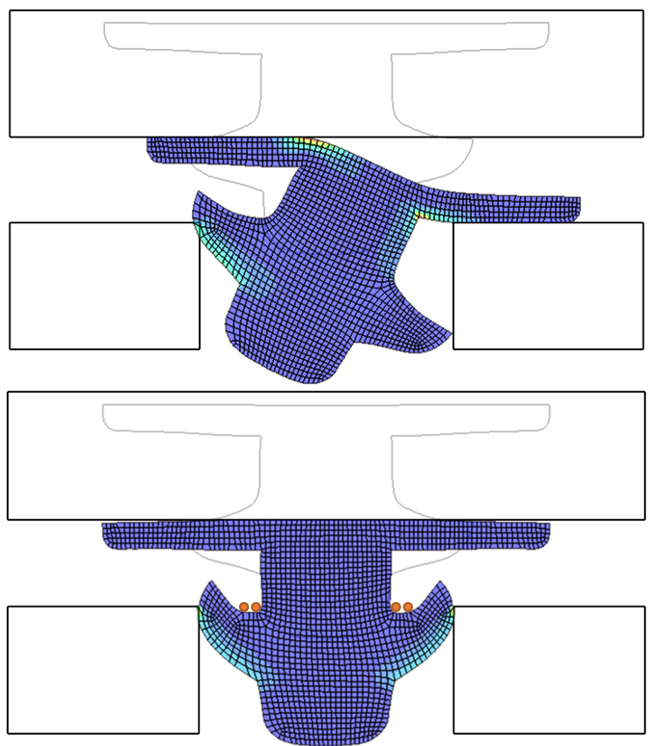
\includegraphics[width=0.54\linewidth]{img/quadsimu/deformation_same_step.PNG}
    \end{figure}
\end{frame}
 
\begin{frame}{Adaptation progressive à la déformation}
    \begin{figure}
        \centering
        \only<1>{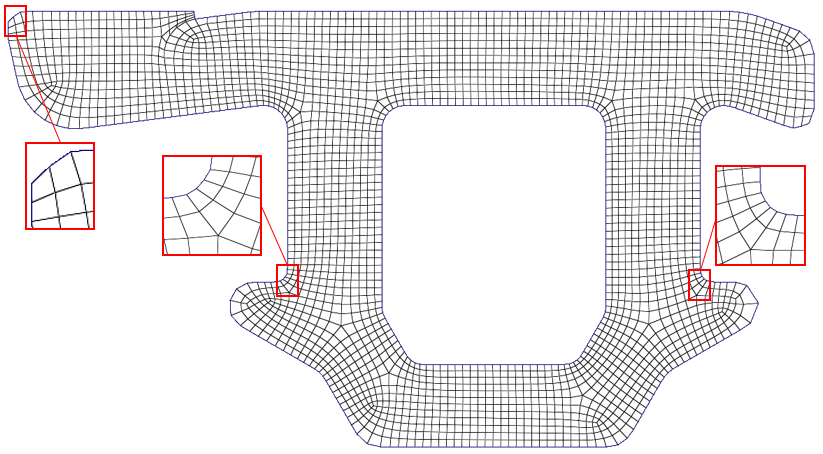
\includegraphics[width=0.69\linewidth]{img/quadsimu/seal_simu_1.PNG}}
        \only<2>{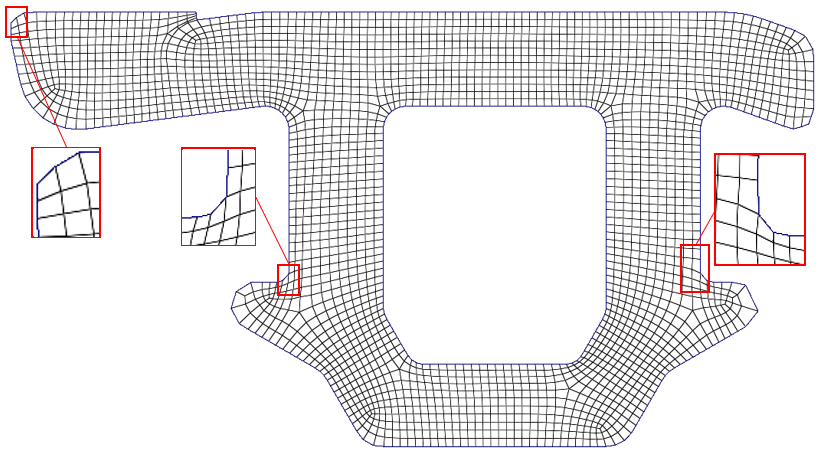
\includegraphics[width=0.69\linewidth]{img/quadsimu/seal_simu_2.PNG}}
        \only<3>{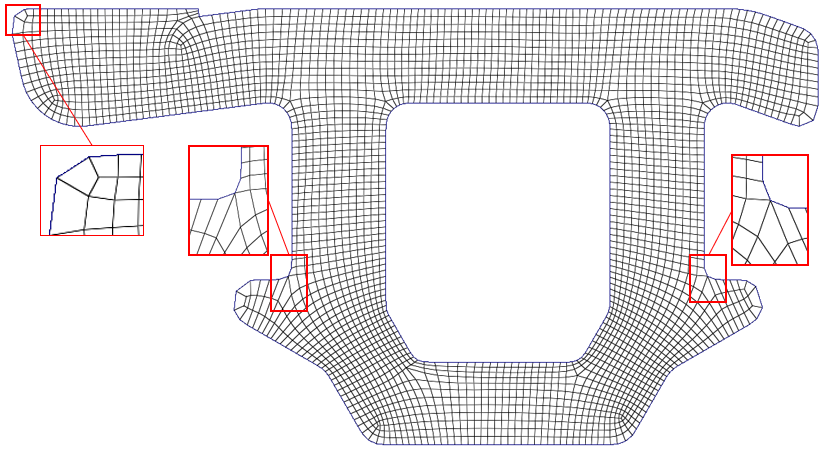
\includegraphics[width=0.69\linewidth]{img/quadsimu/seal_simu_3.PNG}}
    \end{figure}
\end{frame}
